\section{System Architecture} \label{sec:system-architecture}
Our proposed deployment platform comprises four components; pipeline manager, data manager, scheduler, and SGD runner.
Figure \ref{fig:system-architecture} gives an overview of the architecture of our system and the interactions among its components.

\begin{figure}[t]
\centering
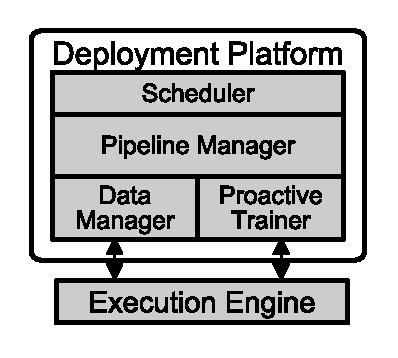
\includegraphics[width=\columnwidth]{../images/system-architecture.pdf}
\caption{System Architecture}
\label{fig:system-architecture}
\end{figure}

\subsection{Scheduler}\label{scheduler}
The scheduler component is responsible for scheduling new iterations of SGD.
The scheduler communicates with pipeline manager to instruct when to execute a new iteration of SGD.
The scheduler allows for two types of scheduling mechanism, namely \textit{static} and \textit{dynamic}.

The static scheduling uses a user-defined parameter that specifies the interval between executions of each iteration of SGD.
This is a simple yet useful mechanism for use cases that require periodical updates of the model when the interval is known a priori (for example, every minute or hour). 
The dynamic scheduling tunes the scheduling interval based on the rate of the incoming prediction, prediction latency, and the time that it takes to execute an iteration of SGD.
The scheduler uses the following formula to compute the time when to execute the next iteration of SGD:
\todo[inline]{This is very simple, does it make sense to include such a thing? specially since in our experiments we are pre setting the incoming prediction throughput.}
\begin{center}
$T' = (2 * T * pr * pl) / pn$
\end{center}
where $T'$ indicates the time in seconds when the next iteration is scheduled to run, $T$ is the execution time of the last SGD iterations, $pl$ and $pr$ are the average prediction latency and number of prediction requests per second, and $pn$ indicates the number of parallel instances of the query answering component.
$T$ is measured by the scheduler component itself while $pr$ and $pl$ are measured by the deployment platform.
$pn$ is determined by the underlying execution engine.
Using the formula to schedule the next SGD iteration, the scheduler ensures that all the prediction requests that arrived during the last SGD iteration and all new prediction requests are answered before a new iteration is scheduled.
Moreover, the scheduler assumes that the entire resources of the computing cluster is being used by the SGD iteration and therefore the prediction answering component is completely blocked while the SGD iteration is being executed.
By removing the above assumption, SGD iterations can be scheduled to execute more frequently.

\subsection{Data Manager} \label{data-manager}
The data manager component is responsible for storage of historical data, processing the incoming training data, and providing the SGD runner with a new batch of training data for every iteration.

Historical data is typically large and may not fit in the memory or disk of a single machine. 
The data manager handles the communication with the underlying storage unit.
When new training data becomes available, the data manager appends the incoming data to the existing historical data.
Moreover, the incoming training data is forwarded to the pipeline manager to update the statistics required by the pipeline components.

When a new iteration of SGD is scheduled to run, the data manager is responsible for providing the batch of training data.
The data manager can provide the next batch of training data in two different modes, namely \textit{sample-then-append} and \textit{append-then-sample}.
In the sample-then-append mode, the new training data that has arrived at the system is stored in an intermediate buffer in the memory.
The historical data is sampled and the resulting data is then combined with the data in the buffer.
The data manager makes the combined data available for the SGD runner to execute the next iteration of SGD.
In the append-then-sample mode, the new training data is appended to the historical data upon arrival.
The data manager then samples the historical data (that consists of the new training data) and provides the resulting dataset for the SGD runner.

The two operation modes of data manager affect the way the deployed model is evolving over time.
In the sample-then-append mode, every iteration of SGD uses the new training data in its entirety.
Therefore, there is more emphasis on the recent data than the historical data.
While this is the more desirable method, it may lead to unstable updates, as the distribution of the data may change due to concept drift or anomalies.
Append-then-sample mode assigns the same weight to every data point (new training and the historical data).
As a result, the update to the deployed model is more stable, however, the increase in model quality is smaller than the sample-then-append mode.
In our experiments, we investigate the effect of the different operation modes on the quality of the model.

%Different sampling strategies can be used to provide the sample.
%In our current prototype, the data manager uses a simple unified random sampling method to generate this sample.
%More advanced methods, such as Reservoir \cite{vitter1985random} or weighted random sampling can also be used to generate the sample.
%Reservoir sampling is typically used to generate samples from large datasets that do not fit in memory, whereas weighted random sampling is used when data elements have different weights.
%In an online machine learning scenario, recent items are more important for training the model and are assigned a bigger weight than older items.
%Therefore, weighted random sampling can generate samples that can contribute to the training of a better model.

Data manager also allows for new training datasets to be registered while the model is being served.
The new dataset is merged with the existing historical data and immediately becomes available for next iterations of SGD.

\subsection{Pipeline Manager} \label{pipeline-manager} 
Pipeline manager is the most important component of the system as it loads the pipeline trained offline, continuously train the pipeline after deployment, evaluate the model update before applying the changes to the deployed model, and exposes the model to answer prediction queries.

Once a pipeline is deployed into the platform, the pipeline manager monitors the pipeline.
The scheduler component informs the pipeline to execute the next SGD iteration.
The pipeline manager then requests the data manager to provide the training dataset for the next SGD iteration.
Once the training dataset is received, the pipeline manager provides the SGD runner component with the current model parameter and training dataset.
Once the SGD iteration is over, the SGD runner sends the updated model back to pipeline manager.
To ensure the quality of the model has not dropped, the pipeline manager uses an independent evaluation set to evaluate the quality of the model.
If the quality of the model does not degrade, the pipeline manager replaces the existing model with the new one.

When new training data arrives at the system, the data manager forwards the data to the pipeline manager. 
The pipeline manager, then, directs the data through the pipeline one component at a time, where each component will receive the data, update their statistics, transform the data, and finally pass the transformed data to the next component.
The model training component of the pipeline is skipped as the model is updated separately in SGD iterations.
If the data materialization is enabled, the data processed by the pipeline is sent back to the data manager to be stored with the rest of the materialized data.
Data manager also forwards prediction requests to the pipeline manager.
Similar to training data, the pipeline manager also sends the prediction request through the pipeline to perform the necessary data processing.
Using the same pipeline to process both the training data and prediction requests guarantees that the same set of transformations are applied to both type of data (training and prediction requests) and prevents inconsistencies between training and serving that is a common problem in model deployment \cite{baylor2017tfx}.
After the prediction request is processed, the pipeline manager uses the model to make a prediction.

\subsection{SGD Runner} 
SGD runner is responsible for executing iterations of SGD.
It is also responsible for tuning the learning rate parameter of SGD.
In every iteration, the SGD runner receives a training dataset and the initial model parameter from the pipeline manager, then performs one iteration of SGD and returns the updated the parameter to the pipeline manager.
Although iterations are independent of each other, SGD runner needs to store the necessary information for computing the learning rate for next iterations.
SGD runner is the only component that is tightly coupled with the execution engine as it directly executes the code on the engine.
Therefore, separate implementations have to be provided for the different execution engines.


\subsection{Execution Engine}
All of the components of our deployment platform described so far, except for SGD runner, are decoupled from the execution engine.
In our deployment platform any data processing platform capable of processing data both in batch mode (for continuous training) and streaming mode (answering prediction requests) is a suitable execution engine.
Apache Flink \cite{carbone2015apache} and Apache Spark \cite{zaharia2010spark} are distributed data processing platforms that can support both stream and batch data processing.
They work with data in memory and on disk which speeds up the execution of SGD iterations.

\textit{Current Prototype.}
In our current prototype, we are using Apache Spark \cite{zaharia2010spark} as the execution engine.
The data manager component uses Hadoop Distributed File System (HDFS) for storing the historical data \cite{shvachko2010hadoop}.
We also leverage some of the components of the machine learning library in Spark to implement the SGD runner.
To enable real-time prediction answering we use Spark streaming \cite{zaharia2013discretized}.
Spark streaming allows us to define the parallelism parameter ($pn$) and extract prediction requests rate and latency ($pr$ and $pl$).
Job scheduler uses these parameters to schedule new iterations of SGD.
